\documentclass{article}
\usepackage{pgfplots}
\usepackage{pgfplotstable}
\usetikzlibrary{calc}
\pgfplotsset{compat = 1.3}
\pgfplotsset{width=0.8\textwidth, height=8cm}
% \pgfmathsetmacro{\YValue}{0.082/0.027}
\begin{document}
\thispagestyle{empty}

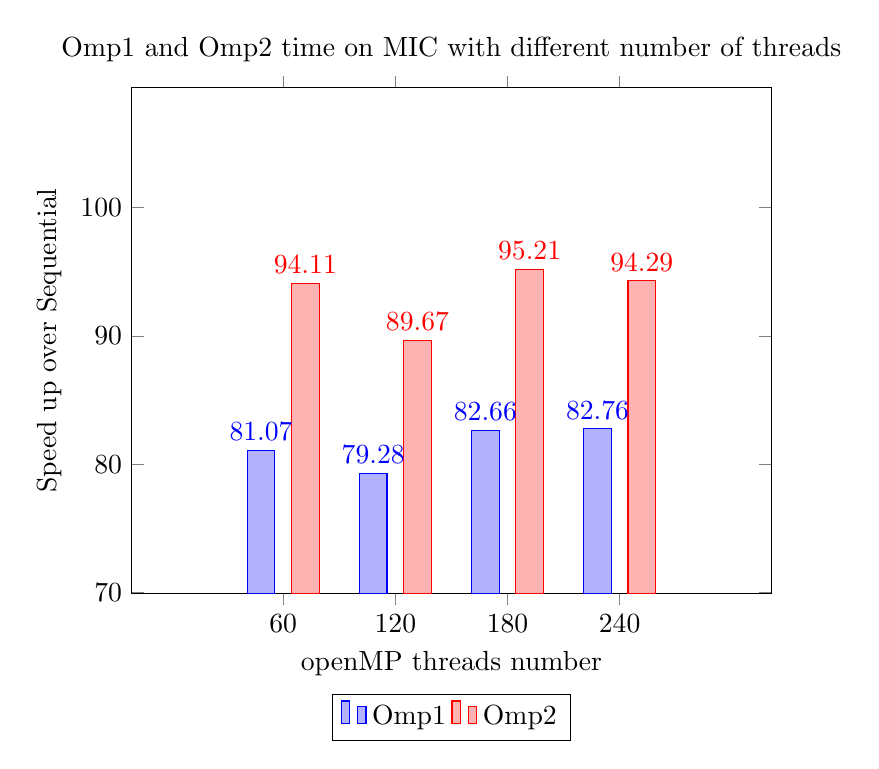
\begin{tikzpicture} \begin{axis}[
	title={Omp1 and Omp2 time on MIC with different number of threads},
	% width=0.8\textwidth,
	% height=8cm,
    ybar=6pt,
	ymax=100,
	enlargelimits=0.45,
	legend style={at={(0.5,-0.2)},
		anchor=north,legend columns=-1},
		ylabel={Speed up over Sequential},
		xlabel={openMP threads number},
		symbolic x coords={60,120,180, 240},
		xtick=data,
		nodes near coords,
		nodes near coords align={vertical},
		]

\pgfkeys{/pgf/fpu=true}
\pgfmathparse{47410/584.813}
\let \spa=\pgfmathresult;
\pgfmathparse{47410/598.037}
\let \spb=\pgfmathresult;
\pgfmathparse{47410/573.578}
\let \spc=\pgfmathresult;
\pgfmathparse{47410/572.876}
\let \spd=\pgfmathresult;
\pgfkeys{/pgf/fpu=false}

\addplot coordinates {(60,\spa) (120,\spb) (180,\spc) (240,\spd)};

\pgfkeys{/pgf/fpu=true}
\pgfmathparse{47410/503.778}
\let \spa=\pgfmathresult;
\pgfmathparse{47410/528.707}
\let \spb=\pgfmathresult;
\pgfmathparse{47410/497.974}
\let \spc=\pgfmathresult;
\pgfmathparse{47410/502.8}
\let \spd=\pgfmathresult;
\pgfkeys{/pgf/fpu=false}

\addplot coordinates {(60,\spa) (120,\spb) (180,\spc) (240,\spd)};

\legend{Omp1, Omp2}
\end{axis}
\end{tikzpicture}

\end{document}
